\documentclass[11pt]{article}
\usepackage{iclr2027_conference}
\iclrfinalcopy
\usepackage{amsmath,amssymb,booktabs,graphicx,hyperref}
\hypersetup{hidelinks}
\setlength{\headheight}{14pt}
\title{OpenVisualJev: Design and Analysis of a Multimodal Decision Model}
\author{Sheng Jin \\ SenseTime Research and Tetras.AI}
\date{}
\begin{document}
\maketitle
\lhead{Technical report --- work in progress}
\begin{abstract}
Multimodal decision models support low-latency decisions by mapping visual context and runtime-defined choices directly to probabilities. We present OpenVisualJev, a vision--language model with tree-masked candidate encoding, permutation-equivariant set interaction, and a dynamic pointer head. Shared image and question prefixes provide context for isolated candidate branches; joint comparison then produces set-dependent scores that remain consistent under candidate reordering. Calibration-aware training and held-out temperature scaling refine these probabilities. Experiments on visual relations, fine-grained recognition, and natural VQA demonstrate order stability, candidate-dependent comparison, and competitive standard-task performance, with larger gains on difficult candidate sets. Ablations identify the contributions of candidate interaction, variable-count training, and calibration. Code is available at \url{https://github.com/jin-s13/OpenVisualJev}.
\end{abstract}
\section{Introduction}
Vision--language models support general-purpose visual understanding, while decision pipelines require low-latency judgments over runtime-defined alternatives. The System One paradigm addresses this requirement through direct probabilistic prediction, extending naturally to image-conditioned decisions~\citep{yu_2026_visualjev,zhou_2026_pixeljev}.

Candidate scoring must accommodate both order symmetry and set dependence: reordering should preserve candidate identity, while changing the alternatives may change relative preferences. Shared encoding and joint comparison combine these properties through set representations~\citep{zaheer_2017_deepsets,lee_2019_set}.

We present OpenVisualJev\footnote{An independently developed research implementation of a Jev-style multimodal decision model.}, which separates candidate grounding from joint comparison. Tree-masked attention shares image and question prefixes across isolated candidate branches in one forward pass. A position-free set module compares their representations, and a shared pointer produces candidate probabilities. Calibration-aware training and held-out temperature scaling complete the model (Figure~\ref{fig:set-pointer-method}).

Controlled order and relation tests examine the architecture's structural properties; unified recognition and natural VQA assess task performance. Ablations isolate candidate interaction, training with variable candidate counts, and calibration.

Our contributions are threefold:
\begin{itemize}
\item A multimodal decision model combining pretrained visual representations, dynamic candidate scoring, and probability calibration.
\item A permutation-equivariant scoring architecture with joint candidate comparison, together with an analysis of its structural properties.
\item Controlled structural tests, recognition and VQA evaluations, and ablations of interaction, candidate-count training, and calibration.
\end{itemize}

\section{Decision interface and model structure}
\begin{figure}[t]
\centering
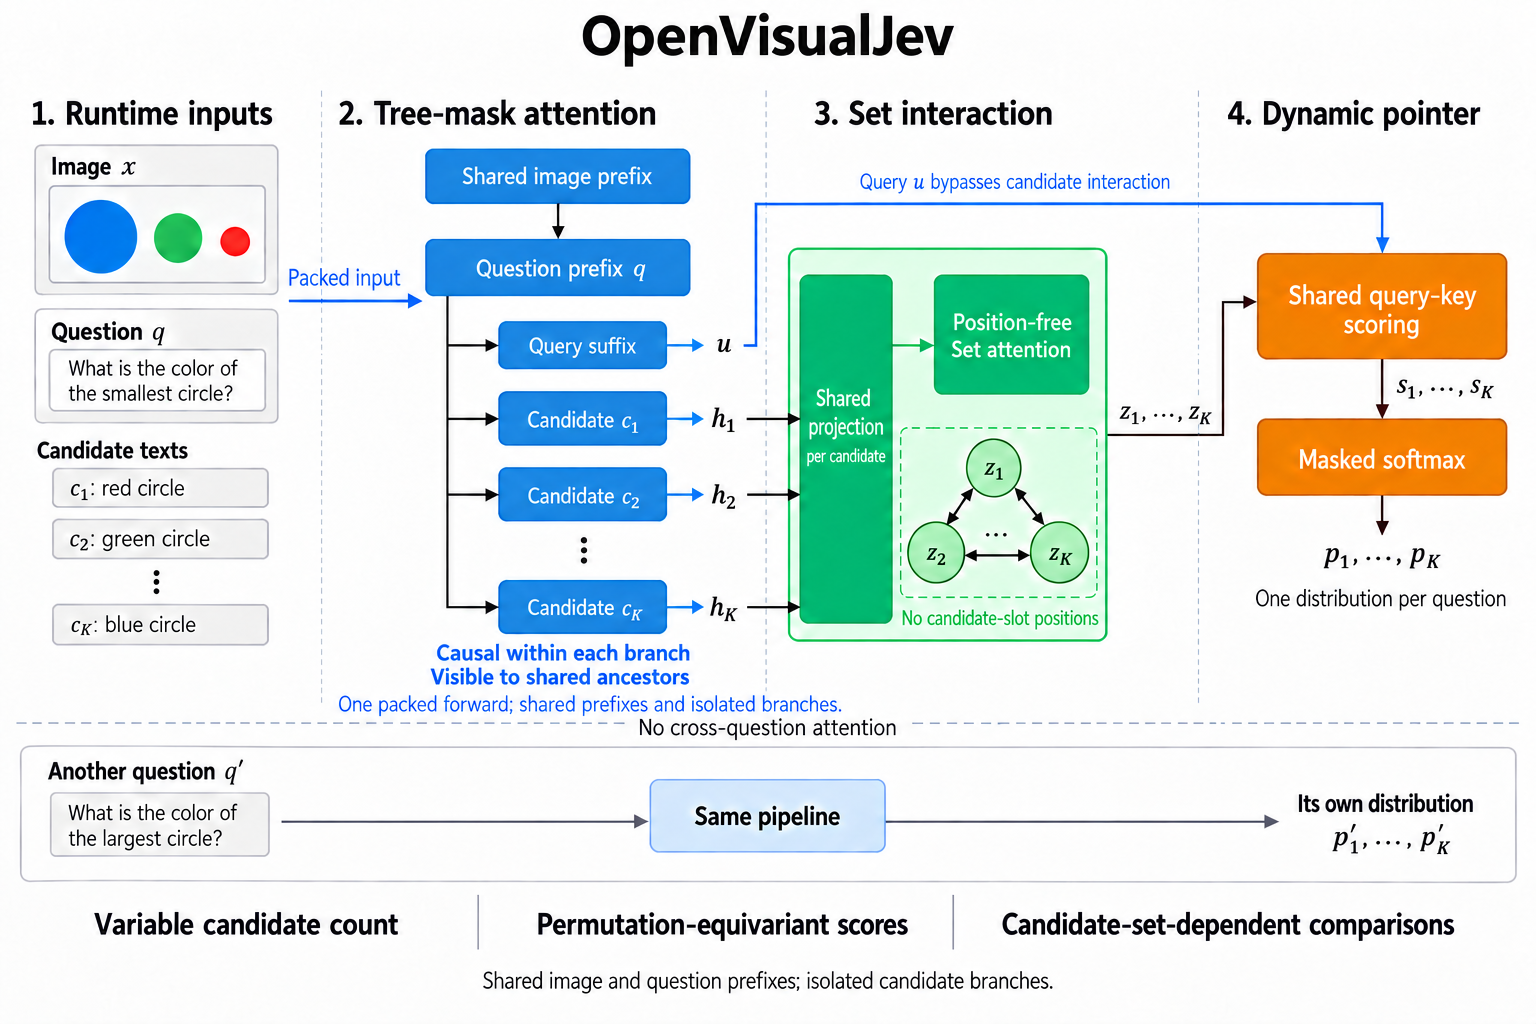
\includegraphics[width=\linewidth]{../figures/set-pointer-method.png}
\caption{OpenVisualJev. Tree-masked attention shares image and question prefixes across isolated query and candidate suffixes. Tokens attend to causal predecessors and ancestors. Position-free Set attention compares candidate representations; the query bypasses this module and scores its outputs through a shared pointer. Interaction and normalization are question-local. Training-time confidence regularization and held-out temperature scaling calibrate the output probabilities.}
\label{fig:set-pointer-method}
\end{figure}

Given an image $x$, a question $q$, and runtime candidate texts $C=(c_i)_{i=1}^{K}$, OpenVisualJev returns a normalized distribution over mutually exclusive candidate slots. External identifiers associate outputs with inputs; prompts contain image, question, and candidate content.

\subsection{Tree-masked multimodal encoding}
The input tree contains a shared image prefix, one prefix per question, and separate query and candidate suffixes. Each prefix appears once. Tokens attend to causal predecessors within their segment and to ancestors; sibling candidates and different questions remain isolated.

\paragraph{Visibility and positions.}
Let $\mathcal A(t)$ contain tokens in the ancestor segments of token $t$, and let $\mathcal C(t)$ contain tokens up to and including $t$ within its own segment. The binary visibility mask is $M_{ts}=\mathrm{I}[s\in\mathcal A(t)\cup\mathcal C(t)]$.
The shared root is causal; a question prefix reads the root and its own history; each leaf additionally reads its question prefix. Masked entries are excluded from attention normalization. Packed offsets only locate tokens in memory: multimodal position coordinates follow the original root-to-leaf sequence. Consequently, placing one candidate before another in the packed sequence creates no additional attention edge between them.

\paragraph{Branch representations.}
Let $E_\theta$ return the final valid-token representation along a root-to-leaf path. The query yields $u=E_\theta(x,q)$, and candidate $i$ yields $h_i=E_\theta(x,q\mathbin{\Vert}\texttt{Candidate:}\mathbin{\Vert}c_i)$. One packed forward computes all leaves, injecting visual features at the shared root. Original branch-local multimodal positions preserve each candidate's coordinates and visible context under reordering.

For multiple questions about one image, each question receives its own internal prefix and leaf group beneath the shared root. Final-token representations are gathered by leaf identity and passed to separate question-local scoring operations. Adding another question therefore adds a disjoint subtree while retaining the existing questions' visible tokens. Candidate count determines the number of leaves and the size of the subsequent set operation; the encoder and pointer parameters are shared across counts.

\subsection{Set interaction and dynamic pointer}
\paragraph{Position-free candidate interaction.}
Stacking candidate representations as rows of $H$, we apply a shared projection and position-free self-attention module $S_\phi$. The query bypasses this module. Scores and probabilities are
\begin{equation}
 Z=S_\phi(H),\qquad s_i=\frac{\langle W_q\operatorname{LN}(u), W_k\operatorname{LN}(Z_i)\rangle}{\sqrt{d}},\qquad p_i=\frac{\exp(s_i)}{\sum_{j\in\mathcal V}\exp(s_j)},
\end{equation}
where $d$ is the query--key dimension and $\mathcal V$ indexes valid slots. Padding is excluded from attention and probability normalization.

\subsection{Structural properties}
\paragraph{Permutation-equivariant scoring.}
Shared row-wise operations commute with a candidate permutation $P$. Consistently permuting query, key, value, and mask gives $\operatorname{Attn}(PH)=P\operatorname{Attn}(H)$; residuals and row-wise normalization preserve this relation. Thus $s(PH)=Ps(H)$ and $p(PH)=Pp(H)$ in exact arithmetic, provided branch preprocessing and positions are unchanged and candidate indices are omitted.

With a unique maximum, the selected candidate identity is preserved under candidate reordering.

The attention relation follows from permuting both axes of the attention matrix: if $A=\operatorname{softmax}(QK^\top/\sqrt d)$, then the permuted matrix is $PAP^\top$. Multiplication by the permuted values $PV$ gives $PAV$. This identity extends through each candidate block, while the shared query remains unchanged. The pointer therefore permutes output slots together with their candidate identities.

\paragraph{Question isolation and candidate-set dependence.}
Tree masking isolates questions, and Set attention and normalization operate within each question. Within a question, logits depend on all candidates, so $p_i/p_j=\exp(s_i-s_j)$ can change when the candidate set changes.

\subsection{Training and probability calibration}
\paragraph{Calibration-aware training.}
We augment cross-entropy with dataset-wise confidence--accuracy alignment, following DCA~\citep{liang_2020_dca}. For dataset groups $B(d)$ in an effective batch, define $a_n=\arg\max_i p_{n,i}$, confidence $c_n=\max_i p_{n,i}$, and correctness $r_n=\mathrm{I}[a_n=y_n]$. Over represented datasets $\mathcal D$, we optimize
\begin{equation}
\begin{aligned}
\mathcal L_{\mathrm{train}}&=\mathcal L_{\mathrm{CE}}+\lambda\mathcal L_{\mathrm{conf}},\\
\mathcal L_{\mathrm{conf}}&=\frac{1}{|\mathcal D|}\sum_{d\in\mathcal D}
\left[\frac{1}{|B(d)|}\sum_{n\in B(d)}\left(c_n-\operatorname{stopgrad}(r_n)\right)\right]^2.
\end{aligned}
\label{eq:training-objective}
\end{equation} Balanced batches weight datasets equally. Gradients flow through confidence while correctness is detached. The loss ablation sets $\lambda=0$ under matched sampling and optimization.

The two loss terms operate at different levels. Cross-entropy supervises each target candidate, whereas the confidence term aligns mean confidence and accuracy within each dataset. Equal group weighting prevents datasets with more examples in an effective batch from dominating that alignment. Post-training temperature fitting then adjusts the frozen model's probability scale on a separate data split.

\paragraph{Reserved probability calibration.}
With model weights frozen, we fit $T>0$ on reserved calibration data by minimizing candidate-event NLL. Predictions use $p_i^{(T)}=\exp(s_i/T)/\sum_{j\in\mathcal V}\exp(s_j/T)$. Scalar scaling preserves ranking, candidate identity, and permutation equivariance.

\section{Experimental setup}
All methods use Qwen3-VL-4B-Instruct~\citep{bai_2025_qwen3vl}, frozen vision parameters, and LoRA on language attention projections~\citep{hu_2021_lora}. Set Pointer and the complete-candidate LM are trained with AdamW~\citep{loshchilov_2017_adamw}, cross-entropy, and the dataset-wise calibration loss. Independent Pointer additionally tests candidate-independent scoring in the relation task. Section~\ref{sec:order-stability} defines the interfaces.

The reported accuracy and probability tables were evaluated with ordinary batched branches using the same branch visibility and positional coordinates described in the method.

\paragraph{Unified recognition.}
One checkpoint per method covers Pets~\citep{parkhi_2012_pets}, CUB, Cars~\citep{krause_2013_cars}, Dogs, Flowers~\citep{nilsback_2008_flowers}, and Aircraft~\citep{maji_2013_aircraft}. Training, development, and calibration contain 31,088, 3,637, and 3,635 images. Testing uses 35,566 FOCI-style four-choice records~\citep{geigle_2024_foci} released with Finedefics~\citep{he_2025_finedefics}, preserving its repeated Dogs row and shuffling candidates identically across methods.

\paragraph{Main model and component ablation.}
The complete models use balanced hard-four-choice training: 96 questions per effective batch, 16 per dataset, seed 20261021, and the epoch-three checkpoint after 2,016 updates. Both receive identical candidate exposures, calibration-loss weight five, and separately fitted temperatures minimizing equal-dataset calibration NLL. Table~\ref{tab:training-calibration} ablates the training penalty and temperature under this recipe; Appendix~\ref{sec:training-calibration-protocol} gives details.

\paragraph{Natural VQA.}
Both interfaces are separately adapted to A-OKVQA~\citep{schwenk_2022_aokvqa} across three seeds and evaluated on 2,576 internal holdout questions. Training, selection, and calibration roles are disjoint (Appendix~\ref{app:essential}).

\paragraph{Metrics.} We report accuracy, NLL, sum-Brier, and ECE with held-out temperature calibration~\citep{guo_2017_calibration}. Recognition weights datasets equally. Paired intervals resample image clusters for recognition and scenes for relations (Appendix~\ref{app:essential}). Bold marks best point estimates, including displayed ties.

\section{Results and analysis}
\subsection{Order stability}
\label{sec:order-stability}
We first test whether the scoring interface preserves candidate identity under changes in presentation order. We compare three scoring interfaces, summarized in Table~\ref{tab:structural-properties}. Their inputs, candidate interactions, and readouts are defined as follows.

\textbf{Independent Pointer} removes the candidate-interaction blocks and scores each independently encoded candidate using a shared 256-dimensional query--key pointer. \textbf{Set Pointer} adds two position-free Transformer blocks (four heads, fourfold feed-forward expansion, GELU, zero dropout), with the query bypassing candidate interaction. \textbf{Complete-candidate LM} encodes all labeled alternatives together and normalizes next-token logits over their single-token labels. All interfaces directly output candidate probabilities; Table~\ref{tab:structural-properties} summarizes their structural properties.

\begin{table}[htbp]
\centering\small
\begin{tabular}{lcc}
\toprule
Interface & Candidate interaction & Equivariant scores \\
\midrule
Independent Pointer & No & Yes \\
Set Pointer & Yes & Yes \\
Complete-candidate LM & Yes & Not guaranteed \\
\bottomrule
\end{tabular}
\caption{Structural properties under the preprocessing and masking conditions in the method. Equivariance is a score property; ties and floating-point effects require separate decision-level checks.}
\label{tab:structural-properties}
\end{table}
For the complete-method checkpoints used in Table~\ref{tab:unified-standard}, LM changes its selected candidate on 108 of 755 questions (14.30\%) across exhaustive permutations; Set changes on none. Each question is evaluated under all 24 candidate orders, yielding 18,120 predictions per model. Predictions are aligned by candidate identity before comparison. Figure~\ref{fig:decision-analysis} connects this order stability to the complete-method performance under larger difficult candidate sets.




\subsection{Candidate interaction enables preference reversals}
Paired three-choice questions share two objects but replace the third with a smaller or larger extreme, reversing the correct median. Candidate-independent utilities cannot reverse the shared objects' ranking. We test fixed checkpoints on 512 fresh scenes (2,048 questions), averaging three training seeds; a largest-object task controls for ordinary ranking.
\begin{table}[htbp]
\centering\small
\begin{tabular}{lrrrrr}
\toprule
& \multicolumn{3}{c}{Median relation} & \multicolumn{2}{c}{Maximum control} \\
Model & Acc. (\%) & Pairs (\%) & NLL & Acc. (\%) & NLL \\
\midrule
Independent & 50.0000 & 0.0000 & 0.70072 & 99.7721 & 0.01175 \\
Set & 99.0234 & 98.3073 & 0.25971 & 99.5768 & 0.03669 \\
Complete LM & 99.7721 & 99.5443 & 0.01878 & 99.8372 & 0.01062 \\
\bottomrule
\end{tabular}
\caption{Fresh-scene test of fixed 80-epoch checkpoints, equally averaging the three retained training seeds. Pairs require both questions correct; all NLL values are uncalibrated. Set and complete-candidate LM both learn the median relation, which requires candidate interaction. The training budget is matched by optimizer updates.}
\label{tab:relation-duration-fresh}
\end{table}

Set resolves the median relation. Independent achieves 99.7721\% accuracy on the maximum control and 0.0000\% paired accuracy on preference reversals. The Set-minus-Independent median-pair difference is 98.3073 percentage points, with paired whole-scene interval $[97.4609,99.0234]$. The complete-candidate LM provides a second interaction-capable reference. The experiment demonstrates the role of candidate-dependent computation. The synthetic test reports raw probabilities.

\subsection{Standard recognition and candidate-count transfer}
\label{sec:unified-recognition}
We evaluate the complete decision model under matched balanced six-dataset training. Both interfaces use cross-entropy plus the dataset-wise calibration loss and a separately fitted temperature. Table~\ref{tab:unified-standard} reports one mixed-dataset model per interface, using the fixed final checkpoint from one shared training seed. Set reaches 90.35\% equal-dataset accuracy versus 90.09\% for LM, a difference of $+0.2690$ percentage points with paired interval $[+0.0086,+0.5317]$.
\begin{table}[htbp]
\centering\small
\begin{tabular}{lrrr}
\toprule
Dataset & LM (\%) & Set (\%) & Difference (pp) \\
\midrule
Pets & 95.88 & 95.42 & -0.46 \\
CUB & 84.52 & 85.57 & +1.05 \\
Cars & 93.74 & 93.83 & +0.09 \\
Dogs & 85.65 & 85.80 & +0.15 \\
Flowers & 99.11 & 98.99 & -0.11 \\
Aircraft & 81.61 & 82.51 & +0.90 \\
\midrule
Equal-dataset mean & 90.09 & 90.35 & +0.27 \\
\bottomrule
\end{tabular}
\caption{Unified mixed-dataset models on author-defined four-choice test records, using the same shuffled candidate sets for both methods. Each method uses one balanced CE-plus-calibration checkpoint across all six datasets, followed by its own held-out temperature. One training seed; differences are Set minus LM, computed before rounding.}
\label{tab:unified-standard}
\end{table}

\paragraph{Transfer to larger difficult candidate sets.}
We evaluate these same complete-method checkpoints at candidate counts of two, four, ten, and twenty, keeping the class inventory fixed. Distractors are selected by the recorded image--text ranking. Table~\ref{tab:full-method-hard} reports equal-dataset accuracy. The Set--LM gap is +0.44 percentage points at four candidates (paired 95\% interval $[+0.17,+0.70]$) and +1.80 points at twenty candidates ($[+1.42,+2.20]$). The larger difficult sets therefore expose a stronger accuracy advantage for Set within this evaluation, while the model is trained with four candidates.
\begin{table}[htbp]
\centering\small
\begin{tabular}{rrrr}
\toprule
Candidates & LM (\%) & Set (\%) & Difference (pp) \\
\midrule
2 & 93.47 & 93.85 & +0.38 \\
4 & 90.10 & 90.54 & +0.44 \\
10 & 84.62 & 86.00 & +1.38 \\
20 & 80.26 & 82.06 & +1.80 \\
\bottomrule
\end{tabular}
\caption{Difficult-candidate count transfer of the complete-method checkpoints in Table~\ref{tab:unified-standard}. Training uses four candidates; test candidates are mined with the fixed image--text ranking. Values are six-dataset mean accuracies from one shared training seed. Differences are Set minus LM.}
\label{tab:full-method-hard}
\end{table}

\subsection{Training with variable candidate counts}
\label{sec:dynamic-k-training}
We test how exposure to variable candidate counts affects performance on larger decision sets. We train each interface with a candidate count sampled independently and uniformly from $K\in\{2,4,10\}$ for each image and epoch. Image exposure, optimizer updates, backbone and development-selection rule are held fixed; the standard four-choice development set still selects the checkpoint. Candidate-token computation varies with the sampled count. The test candidate sets are identical across all four checkpoints, and twenty candidates remain outside the training support. The category inventory is held fixed while candidate count varies.
\begin{table}[htbp]
\centering\small
\begin{tabular}{lrrrr}
\toprule
Test & LM fixed & Set fixed & LM variable & Set variable \\
\midrule
Standard & 89.08 & 89.79 & 89.08 & 89.82 \\
Hard 2 & 92.87 & 93.36 & 92.73 & 93.26 \\
Hard 4 & 89.25 & 89.93 & 89.13 & 89.91 \\
Hard 10 & 84.94 & 86.27 & 86.02 & 87.24 \\
Hard 20 & 82.01 & 84.47 & 84.20 & 85.82 \\
\bottomrule
\end{tabular}
\caption{Equal-dataset accuracy (\%) for fixed four-candidate training and variable-candidate training. All four models use the same single training seed and test records. Difficult-distractor tests and the author-defined standard test are separate constructions.}
\label{tab:dynamic-k-training}
\end{table}
At twenty difficult candidates, the change from fixed to variable training is +2.19 [+1.86, +2.53] percentage points for LM and +1.35 [+1.08, +1.62] for Set (paired image-bootstrap intervals). The corresponding change in the Set--LM gap is -0.85 [-1.25, -0.45] percentage points. These comparisons condition on the selected weights and assess the variable-count training recipe, including its candidate-token computation.
Both methods improve at larger difficult candidate counts, but LM benefits more at twenty candidates, narrowing the Set--LM gap. Set retains a positive gap of +1.62 [+1.31, +1.93] percentage points after variable-count training. Thus the magnitude of the fixed-count advantage depends partly on training exposure. Standard-test point estimates remain close to their fixed-count counterparts. On the same exhaustive-order subset, the variable-count Set still has no decision changes, whereas the variable-count LM still changes candidate identity. The permutation test distinguishes the order behavior of the two interfaces after variable-count training.


\subsection{Training and post-training calibration}
Table~\ref{tab:unified-probability} evaluates the probability outputs of the complete-method checkpoints. Independently fitted temperatures reduce NLL and Brier for both interfaces while preserving their decisions. After calibration, Set has NLL 0.2831 versus 0.2778 for LM; the paired Set-minus-LM difference is $+0.00530$ with interval $[+0.00004,+0.01054]$. Set has a lower Brier point estimate, 0.1428 versus 0.1438, with difference $-0.00105$ and interval $[-0.00356,+0.00148]$. Figure~\ref{fig:calibration-analysis} visualizes how temperature scaling changes the confidence--accuracy relationship within each dataset.
\begin{table}[htbp]
\centering\small
\begin{tabular}{lrrrr}
\toprule
& \multicolumn{2}{c}{Raw} & \multicolumn{2}{c}{Temperature-scaled} \\
\cmidrule(lr){2-3}\cmidrule(lr){4-5}
Metric $\downarrow$ & LM & Set & LM & Set \\
\midrule
NLL & 0.3008 & 0.3478 & 0.2778 & 0.2831 \\
Sum-Brier & 0.1473 & 0.1480 & 0.1438 & 0.1428 \\
ECE & 0.0337 & 0.0448 & 0.0224 & 0.0355 \\
\bottomrule
\end{tabular}
\caption{Equal-dataset mean probability metrics for the balanced CE-plus-calibration checkpoints in Table~\ref{tab:unified-standard}. ECE uses fifteen equal-count bins and is descriptive. Lower is better. Calibration uses post-training temperature scaling.}
\label{tab:unified-probability}
\end{table}


\begin{figure}[htbp]
\centering
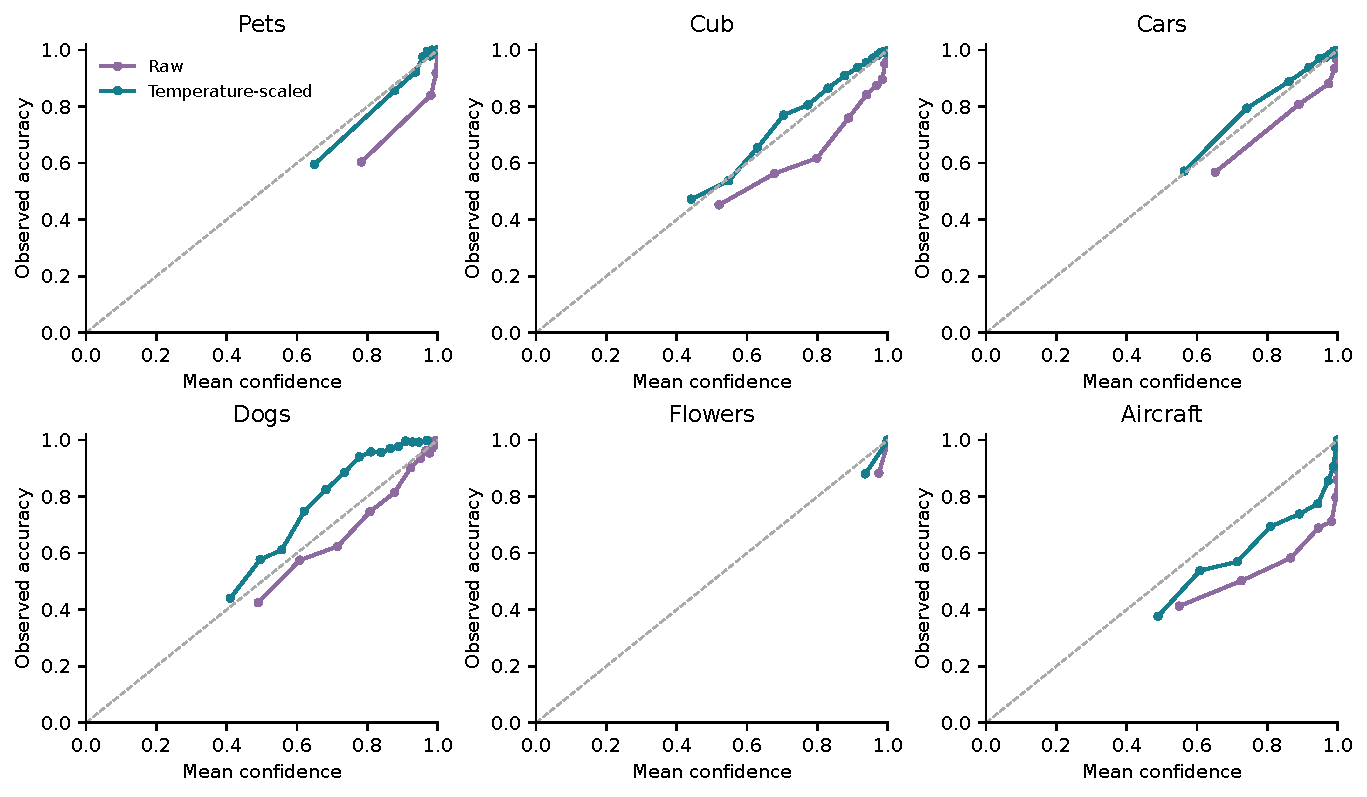
\includegraphics[width=\linewidth]{../figures/calibration-analysis.pdf}
\caption{Probability calibration of the complete Set model on the six recognition datasets. Each curve uses fifteen equal-count confidence bins; points show mean top-choice confidence and observed accuracy. The dashed diagonal denotes matched confidence and accuracy. Temperature scaling uses the single scalar fitted on the reserved calibration data, with unchanged predictions.}
\label{fig:calibration-analysis}
\end{figure}

\paragraph{Training-time calibration.}
We further compare cross-entropy training with a dataset-wise mean-confidence penalty under a matched, balanced six-dataset training recipe. Both Set models use the same seed, candidate exposures, and final-epoch checkpoint. Table~\ref{tab:training-calibration} shows that the penalty improves raw NLL, Brier, and ECE while changing macro accuracy from 90.48\% to 90.35\%. Fitting a separate temperature for each model by minimizing equal-dataset calibration NLL further improves probability quality: NLL decreases from 0.2985 to 0.2831 and Brier from 0.1457 to 0.1428 when the training penalty is added. The paired NLL difference is $-0.01539$ with interval $[-0.01953,-0.01142]$; the accuracy difference is $-0.1273$ percentage points with interval $[-0.3205,+0.0676]$. These results support combining the training penalty with post-training temperature scaling. Appendix~\ref{sec:training-calibration-protocol} specifies the matched training recipe.
\begin{table}[htbp]
\centering\small
\begin{tabular}{llrrrr}
\toprule
Training & Probability & Accuracy (\%) & NLL $\downarrow$ & Brier $\downarrow$ & ECE $\downarrow$ \\
\midrule
CE & Raw & 90.48 & 0.4003 & 0.1519 & 0.0521 \\
CE + calibration & Raw & 90.35 & 0.3478 & 0.1480 & 0.0448 \\
CE & Temperature & 90.48 & 0.2985 & 0.1457 & 0.0427 \\
CE + calibration & Temperature & 90.35 & 0.2831 & 0.1428 & 0.0355 \\
\bottomrule
\end{tabular}
\caption{Training-loss comparison for Set under balanced six-dataset training with one shared seed. Metrics are equal-dataset means on the standard test; Brier is summed over candidates and ECE uses fifteen equal-count bins. Each model receives its own held-out temperature fitted with an equal-dataset NLL objective. Positive scalar temperature scaling preserves accuracy.}
\label{tab:training-calibration}
\end{table}


\subsection{Natural VQA performance}
On A-OKVQA, Set remains close to the native LM, with an accuracy decrease of 0.53 points across three seeds (Table~\ref{tab:vqa-native-summary}; exploratory interval $[-1.7041,0.6406]$). Scaled probability losses favor LM. This test evaluates retention of general VQA capability; split and uncertainty details are in Appendix~\ref{app:essential}.
\begin{table}[htbp]
\centering\small
\begin{tabular}{lrrr}
\toprule
Interface & Accuracy (\%) & Scaled NLL & Scaled Brier \\
\midrule
Native LM & 87.2800 & 0.3703 & 0.1845 \\
Set & 86.7495 & 0.3819 & 0.1932 \\
\bottomrule
\end{tabular}
\caption{Natural VQA capability and calibrated probability quality, using the completed supervised holdout experiment. Means use all registered seeds and frozen, independently fitted temperatures. The comparison follows the registered native-LM secondary analysis. Raw probability differences and protocol details appear in Appendix~\ref{app:essential}.}
\label{tab:vqa-native-summary}
\end{table}


\section{Related work}
\label{sec:related}
\paragraph{Multimodal decision models.}
Recent Jev-style systems map runtime-defined alternatives to probabilities. Visual Jev and PixelJev adapt vision--language models using option-token readouts~\citep{yu_2026_visualjev,zhou_2026_pixeljev}, while Koa-action learns atomic label tokens with randomized label mappings~\citep{dai_2026_koa}. OmniJev combines learned option scoring with probabilistic supervision and calibration~\citep{xu_2026_omnijev}, and Chinese-Jev develops a text-encoder decision model with heterogeneous supervision~\citep{wang_2026_chinesejev}. Shared-context execution provides a complementary systems direction: Visual Jev reuses image prefixes, and FastJEV studies state reuse and candidate-layer pruning~\citep{yu_2026_visualjev,ma_2026_fastjev}. OpenVisualJev focuses on the scoring architecture, combining independent candidate representations with explicit, permutation-equivariant joint comparison.

\paragraph{Set-dependent choice.}
Deep Sets establishes invariant and equivariant set representations, and Set Transformer models interactions through attention~\citep{zaheer_2017_deepsets,lee_2019_set}. Context-dependent choice models such as FETA and FATE allow an alternative's utility to depend on the surrounding set, including preference reversals when another alternative changes~\citep{pfannschmidt_2019_context}. Our candidate module applies these principles to multimodal representations. The relation experiments test this capacity directly, alongside the stability of scores under candidate permutations.

\paragraph{Probability quality and decision evaluation.}
Jev benchmarks and decision-gate studies examine calibration, selective prediction, option ordering, and candidate-count robustness~\citep{deusser_2026_benchmark,rafe_2026_gates}. Judge routing, security screening, and mobile action selection illustrate the downstream use of decision scores~\citep{li_2026_jevjudge,liu_2026_security,zhang_2026_jevmobile}. Visual MCQA debiasing and selective VQA likewise connect answer confidence with reliable selection~\citep{atabuzzaman_2025_bias,eisenschlos_2024_selective}. Our evaluation separates recognition accuracy, order stability, and probability quality. The calibration pipeline builds on confidence--accuracy regularization and multiclass calibration objectives~\citep{liang_2020_dca,hebbalaguppe_2022_mdca}, followed by temperature scaling~\citep{guo_2017_calibration}; ablations measure the contributions of training-time and post-training adjustment.

\paragraph{Fine-grained visual recognition.}
FOCI formulates fine-grained recognition as multiple-choice answering with difficult distractors~\citep{geigle_2024_foci}. Finedefics combines attribute-mediated alignment with classification instruction tuning~\citep{he_2025_finedefics}. We reuse the candidate records released with the Finedefics evaluation code and train a unified Qwen3-VL model across six datasets. This provides a common recognition setting for comparing scoring architectures and complements the controlled structural experiments.

\section{Conclusion}
OpenVisualJev combines tree-masked multimodal encoding, position-free set interaction, dynamic pointer scoring, calibration-aware training, and held-out temperature scaling into a multimodal decision pipeline. The design combines permutation-equivariant scores with preferences conditioned on the candidate set. Exhaustive permutations verify decision stability, and preference-reversal tasks demonstrate the expressive role of candidate interaction. Under the evaluated single-seed balanced protocol, Set achieves higher macro accuracy than the complete-candidate LM across six recognition datasets; dynamic candidate-count training improves both models on larger candidate sets. Separately supervised natural VQA yields accuracy close to the native LM. The balanced training-loss ablation supports combining mean-confidence regularization with temperature scaling to improve probability quality. These findings identify candidate-set structure as a useful design principle for multimodal decision models and provide an empirical basis for its use in dynamic choice tasks.

\label{main-text-end}
\bibliographystyle{iclr2027_conference}
\bibliography{references}
\section*{AI usage disclosure}
Generative AI assisted this research under the author's direction, using the open-source \href{https://github.com/jin-s13/ai-research-writing-skill}{\texttt{ai-research-writing-skill}} workflow. Assistance covered literature review, method and experiment design, implementation and debugging, analysis, figures, and manuscript preparation. Synthetic relation data were produced by executable generation code; reported results were computed from model predictions and checked against evaluation artifacts. The author reviewed the work and retains responsibility for its claims, code, data, and figures.

\appendix
\section{Essential reproducibility details}
\label{app:essential}
\paragraph{Recognition data and optimization.}
Pets, CUB, Cars, and Dogs reserve development/calibration images within classes from the official training-side inventory. Flowers and Aircraft use official validation images for those roles. Exact and reviewed near-duplicate groups are separated from test-side images; additional cross-dataset exclusions precede mixed training. The duplicate audit covers the task-specific training and evaluation inventories. The six datasets contain 37, 200, 196, 120, 102, and 100 classes, respectively; the choice count is independent of class count.

FOCI/Finedefics test candidate sets are preserved, including the original repeated Dogs row, and shuffled consistently across methods. The unified protocol follows the released Dogs test inventory. Training and dynamic tests mine difficult incorrect labels with the recorded OpenCLIP ViT-L-14 image--text ranking; random distractors are distinct sampled incorrect classes. The correct label is included. The standard author-defined four-choice test and the newly constructed difficult four-choice test are separate conditions.

Unified training uses learning rate 0.0001, accumulation over eight questions, three epochs, cosine decay, warmup fraction 0.03, AdamW weight decay 0.01, global clipping at norm one, and language-attention LoRA rank/scaling 16/32. The seed is 20261021. Both methods use candidate-conditioned cross-entropy, the same exposure and selection rule, and development-based checkpoint selection. Variable-count training changes only the registered candidate-count sampling and associated candidate construction; candidate-token computation follows the sampled candidate counts. Images use processor area bounds 65536 and 262144 pixels; Aircraft crops the bottom twenty pixels. Other recognition images are uncropped.

\paragraph{Relation construction and endpoint.}
Images contain colored objects with distinct sizes. Paired three-choice questions share two middle objects but replace the third candidate with a smaller or larger extreme, reversing the median answer. The largest-object task serves as an independent-ranking control.  Whole-scene bootstrap intervals condition on those trained seeds.

\paragraph{VQA comparison scope.}
The main text presents the registered native-LM secondary comparison. The original primary contrast used a canonically sorted LM input: Set-minus-canonical-LM accuracy was $-0.5694$ percentage points, with conditional interval $[-1.2861,0.1289]$. The original primary and secondary analysis roles are retained. For native LM, raw Set-minus-LM NLL and Brier differences are $+0.1933$ and $+0.0243$; their exploratory crossed intervals are $[0.0779,0.3260]$ and $[0.0078,0.0407]$. Scaled differences are $+0.0116$ for NLL and $+0.0087$ for Brier, with crossed intervals $[-0.0054,0.0284]$ and $[-0.0025,0.0204]$. The registered analysis estimates accuracy and probability-loss differences with intervals.

\paragraph{Calibration and statistical conventions.}
Recognition minimizes reserved-set pooled candidate NLL over $\log T\in[-5,5]$ using bounded scalar optimization and explicit boundary checks. VQA uses a fixed grid of 2001 log-temperatures in the same range, preferring the value closest to zero on objective ties. Temperatures are fixed before test scoring. Sum-Brier sums squared probability errors across candidate or literal-answer events. Recognition ECE uses fifteen equal-count bins; VQA uses fifteen equal-width bins. Exact score ties are resolved by selecting the first slot. Paired bootstrap samples keep repeated images and related questions together. The recognition and relation intervals condition on the trained seeds; the crossed VQA analysis is exploratory with few training realizations. All intervals are conditional on the fitted temperatures and the evaluation distribution.

\paragraph{Reproduction scope.}
The recorded implementation uses PyTorch 2.8.0, Transformers 4.57.3, PEFT 0.17.1, and NVIDIA A800 devices. Data manifests, model checkpoints, raw predictions, and analysis scripts provide the evidence trail. The project archive preserves earlier specialist adapters, intermediate training endpoints, optimization probes, and engineering validation records. Public external reproduction remains a planned release milestone.

\subsection{Equivalent answer events}
For the registered VQA protocol, blank and duplicate candidate strings are preserved. Prediction selects the maximum-logit slot, with first-slot tie breaking, before comparison by literal answer text. For probability scoring, the mass of identical strings is summed. Given a gold answer event $G$, the candidate-conditioned loss is
\begin{equation}
 \mathcal L=-\log\sum_{i\in G}p_i
 =\operatorname{LSE}_{j\in\mathcal V}(s_j)-\operatorname{LSE}_{i\in G}(s_i).
\end{equation}
Labels supply supervision to the loss and evaluator; forward prompts contain the image, question, and candidate text. This convention preserves the official answer-text task while keeping slot and answer-event probabilities distinct.

\subsection{Supplementary evaluation details}
\paragraph{Candidate-count study.}
The variable-count training ablation uses a separate unified CE recipe: three epochs with matched image exposure, alternating difficult and random distractors, and development selection by equal-dataset accuracy with earlier-epoch tie-breaking. Fixed-count training uses four candidates; variable-count training samples uniformly from $K\in\{2,4,10\}$. The reported count-transfer tests use difficult distractors at two, four, ten, and twenty candidates alongside the standard records. The four checkpoints share the training seed and test manifests. This study matches image exposure and updates; candidate-token computation varies with candidate count. Twenty-candidate testing measures transfer beyond the training count range.

\paragraph{Order and relation tests.}
The order test evaluates all 24 permutations of four candidates on 755 class-stratified questions, aligning candidate identities before comparison. Both this test and the difficult-candidate count-transfer evaluation use the complete-method checkpoints from Table~\ref{tab:unified-standard}, with unchanged weights and inference precision. Relation tests use synthetic scenes with paired candidate sets that reverse the required preference between shared objects. Independent, Set, and complete-candidate LM are evaluated with three training seeds at the same fixed final training endpoint on fresh scenes. The paired metric requires both questions correct; a largest-object control tests ordinary independent ranking.

\paragraph{Probability quality and uncertainty.}
Each model receives its own scalar temperature fitted only on reserved calibration data~\citep{guo_2017_calibration}. We report accuracy, NLL, sum-Brier, and ECE, distinguishing raw and scaled probabilities. Recognition ECE uses fifteen equal-count bins; the VQA protocol uses equal-width bins over literal answer events. Recognition intervals use 10,000 paired image-cluster bootstrap replicates within datasets and equal dataset weighting; repeated image rows stay together. They condition on the selected weights and fitted temperatures, excluding training-seed and calibration-fit uncertainty. Relation intervals resample whole scenes; the VQA interval additionally resamples the few available seeds and is exploratory. Intervals are marginal, without multiplicity correction. Further protocol details appear in Appendix~\ref{app:essential}.

\end{document}
